
\section{Gestión de producción}
\subsection{Autoevaluación}
En esta sección se ha cumplido los objetivos correspondientes al 10.
\subsection{Introducción}
\paragraph{}
La gestión de fabricación es una parte importante en el proceso de producción de las empresas, y Odoo ofrece un conjunto de módulos diseñados para gestionarlo. Odoo nos permite programar y controlar el proceso de fabricación de productos. Además, facilita el seguimiento y la gestión de los movimientos de inventario, la recepción de materias primas, el almacenamiento de productos en almacenes y permite la gestión de todo el proceso de las compras.
\subsection{Metodología}
\paragraph{}
Para llevar a cabo la gestión de la fabricación en Odoo, se ha instalado los módulos de \textit{Fabricación}, \textit{Inventario} y \textit{Compras}. A continuación, se han realizado cambios en los ajustes para adaptar estos módulos a nuestras necesidades. Se ha activado en ajustes del módulo Inventario la opción \textit{Ubicaciones de almacenamiento} y \textit{Rutas multietapa} y en el módulo de Fabricación se ha activado la opción \textit{Ordenes de trabajo}. 
\paragraph{}
La empresa CochesMA se ocupa de la venta de vehículos. Para ello, desde el módulo de Fabricación y en el menú de Productos se ha creado un producto llamado Coche Mini completando la información referente al producto y este producto solo puede ser vendido y se obtendrá mediante su fabricación. Los otros 3 productos también se han creado pero en este caso solo pueden ser comprados y se obtendrán mediante la compra. A continuación, en el menú de lista de materiales se crea una nueva entrada donde se ha definido que el coche se fabricará con los siguientes productos: 4 \textit{Ruedas}, un \textit{Motor} y un \textit{Chasis}. 
\paragraph{}
Para probar que se ha puede realizar la fabricación manual de un producto, primero se ha comprado la cantidad necesaria de los tres productos desde el menú \textit{A mano} dentro de cada producto, actualizando su cantidad. Tras esto, desde el producto del Coche Mini se hace click en reponer y como consecuencia se habrá generado una orden de fabricación. Si se accede a esta orden y se confirma esta operación, se puede ver que la lista de productos se ha generado un coche y se han consumido los materiales necesarios para su fabricación. 
\paragraph{}
También, se pueden distribuir los productos y materiales en distintos almacenes, para probarlo se han creado 2 almacenes nuevos. De esta manera tenemos el almacén principal \textit{CochesMA} y los dos nuevos, \textit{CochesMA - almacén 2} y \textit{CochesMA - almacén 3}. Se ha definido que se va a almacenar las ruedas en el almacén 2, los motores en el almacén 3 y tanto los coches fabricados como los chasis en el almacén principal. Cuando se necesite realizar la fabricación de un coche las ruedas y los motores necesarios se trasladarán al almacén principal donde junto al chasis se procederá a fabricar el coche. Además, se ha automatizado la acción de comprar los productos cuando se acaben y de trasladarlos al almacen principal para su fabricación. Para ello, se han utilizado las reglas de reabastecimiento de la siguiente manera:
\begin{figure}[h]
    \centering
    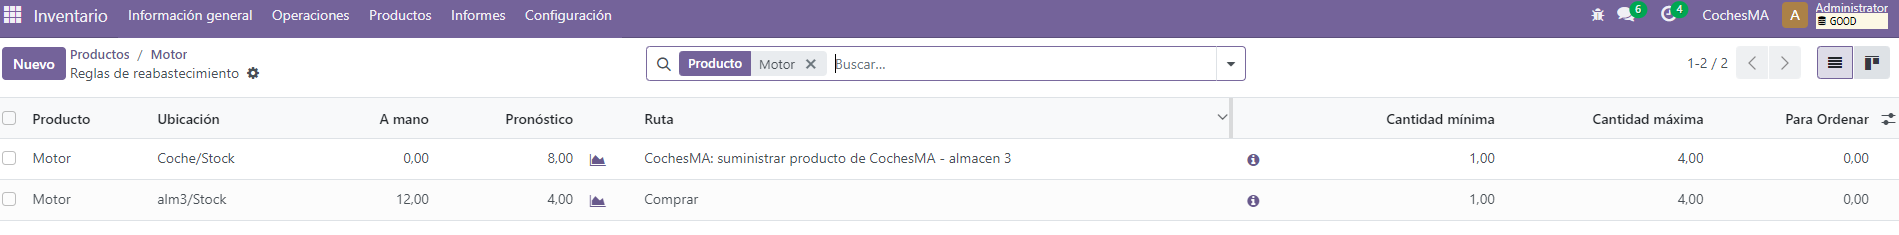
\includegraphics[width=1\linewidth]{fotosGestFab/ruedas.png}
    \caption{Reglas de reabastecimiento de las ruedas}
    \label{fig:enter-label}
\end{figure}
\paragraph{}
También se ha automatizado la fabricación de los vehículos por lo que cuando haya un pedido de un vehículo si no hay existencias se comenzará con la fabricación del mismo. 
\subsection{Resultados y análisis}
\paragraph{}
En este apartado se ha evaluado la capacidad de gestionar la fabricación que ofrece Odoo mediante los módulos de Fabricación, Inventario y Compras. Se han hecho configuraciones para personalizar estos módulos a las necesidades de las pruebas que se querían realizar. Además, se ha creado el producto Coche Mini que tiene una lista de materiales con los que se fabricará, 4 ruedas, un chasis y un motor.
\newpage
\begin{figure}[h]
    \centering
    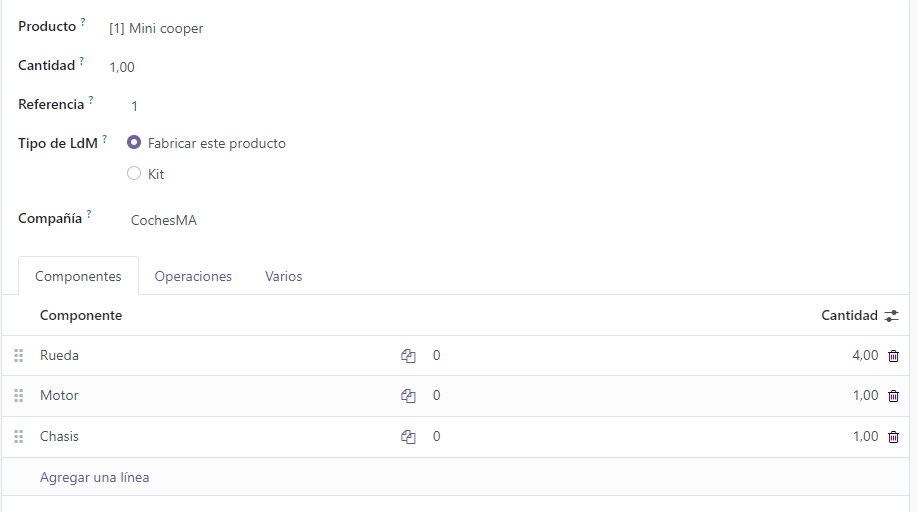
\includegraphics[width=1\linewidth]{fotosGestFab/coche.png}
    \caption{Lista de materiales de un coche Mini}
    \label{fig:enter-label}
\end{figure}
\paragraph{}
Se ha realizado la fabricación de un coche Mini de forma manual.
\begin{figure}[h]
    \centering
    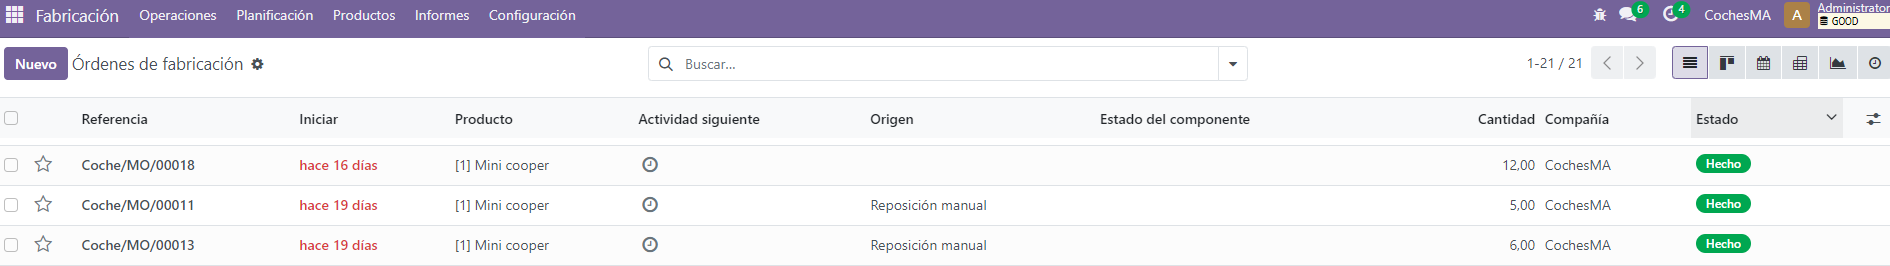
\includegraphics[width=1\linewidth]{fotosGestFab/manual.png}
    \caption{Orden de fabricación de un coche Mini de forma manual}
    \label{fig:enter-label}
\end{figure}
\paragraph{}
A continuación, se ha automatizado la compra y transferencia de productos entre almacenes para cumplir con la producción necesaria.
\begin{figure}[h]
    \centering
    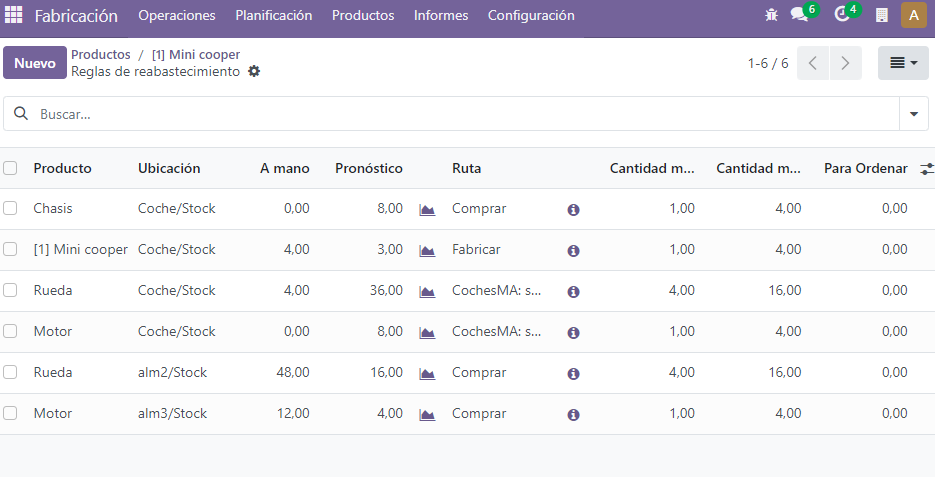
\includegraphics[width=1\linewidth]{fotosGestFab/reabastecimiento.png}
    \caption{Orden de reabastecimiento de los productos}
    \label{fig:enter-label}
\end{figure}
\newpage
\paragraph{}
Por último, se ha realizado un diagrama BPMN (figura \ref{fab}), el cual describe cómo se realiza el proceso de fabricación de un coche.
\begin{figure}[h]
    \centering
    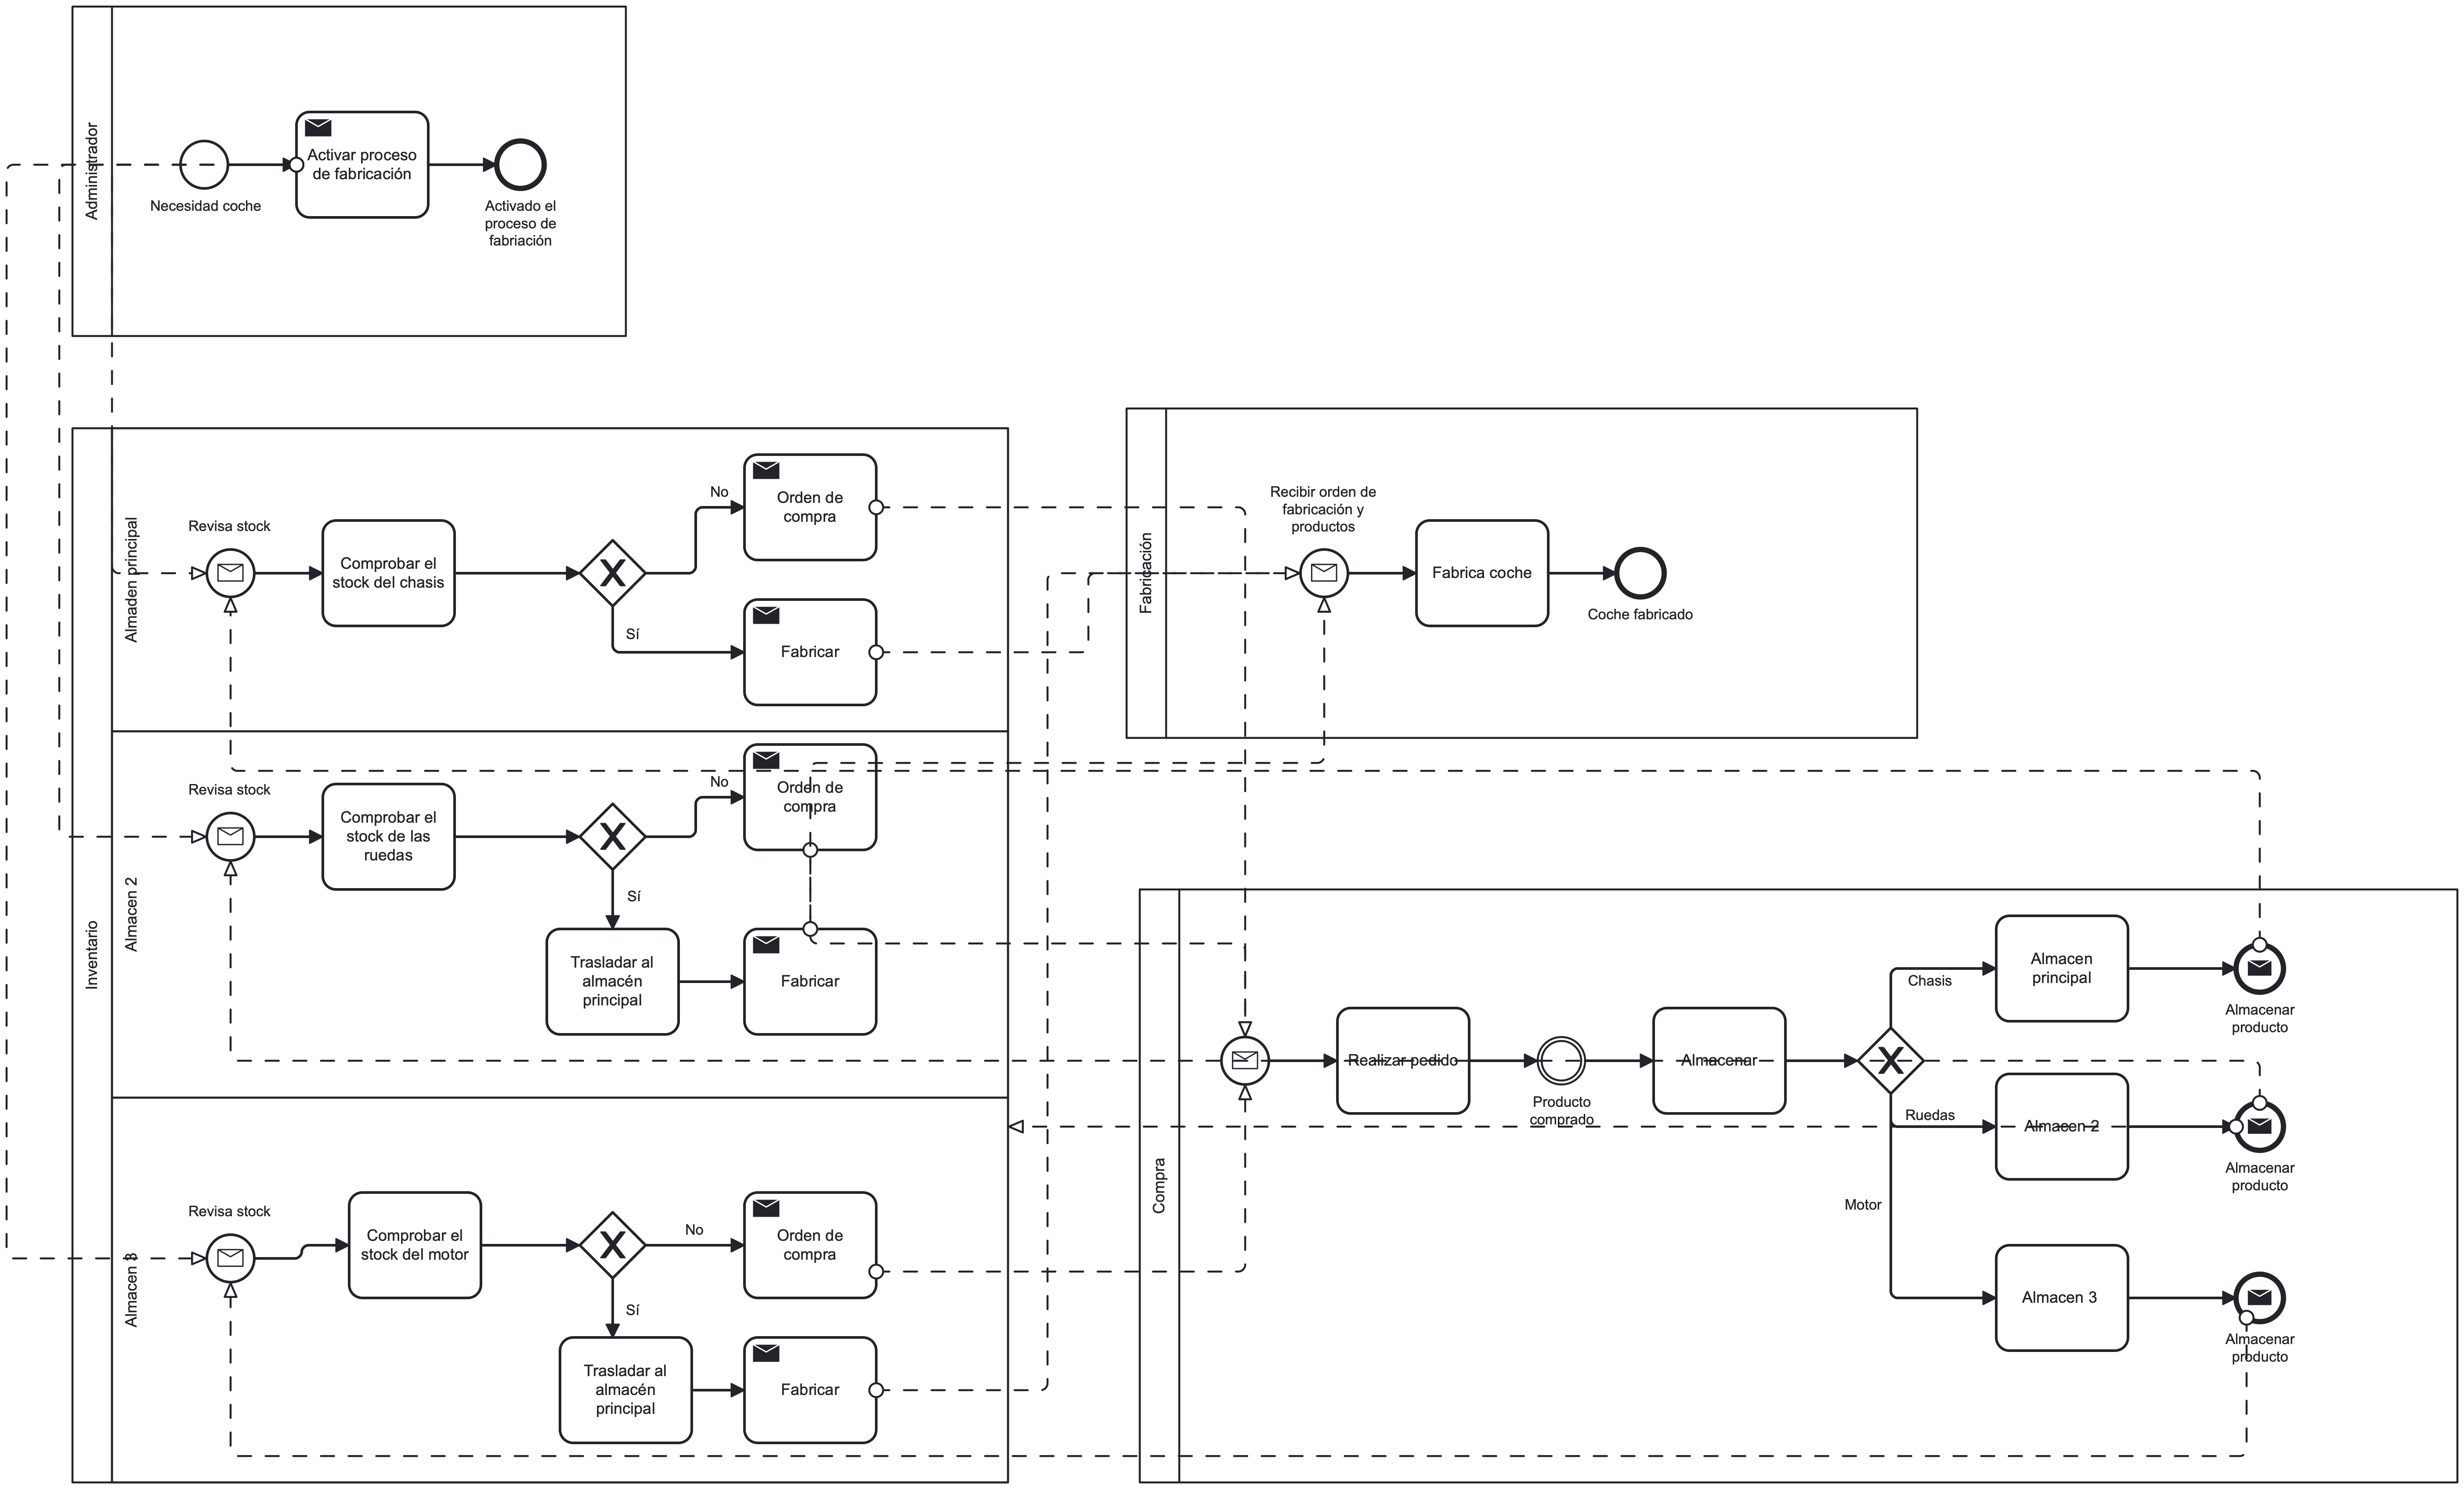
\includegraphics[width=1\linewidth]{fotosGestFab/Fabricacion.png}
    \caption{Diagrama BMPN 2.0 del proceso de fabricación}
    \label{fab}
\end{figure}
\subsection{Conclusiones}
\paragraph{}
La gestión de la fabricación en Odoo ofrece una gran cantidad de herramientas para controlar y optimizar el proceso de producción. Sin embargo, durante la realización de las pruebas y configuraciones, se han detectado tareas complejas como la automatización de las reglas de abastecimiento. Además, puede ser dificil de configurar correctamente para usuarios novatos porque el proceso de gestión de almacenamientos puede resultar confusa. Se recomienda proporcionar una formación adecuada a los empleados que se dediquen a este sector ya que es complicado de gestionar pero Odoo ofrece unas funcionalidades con un gran potencial, que permitirá optimizar en tiempo la gestión de los productos, su fabricación y su ubicación.